% A Numerical Comparison of Explicit Euler, a Velocity-Verlet-type Scheme,
% and RK4 for the Damped Harmonic Oscillator
% Draft v0.1 (2026-09-29). Author: Yi Zhou.
% Figures are generated from saved CSV data; see ../README.md for the
% reproduction pipeline. Compile with: pdflatex main.tex

\documentclass[11pt,a4paper]{article}

\usepackage{amsmath,amssymb}
\usepackage{graphicx}
\usepackage{booktabs}
\usepackage{hyperref}
\usepackage[margin=2.5cm]{geometry}

\title{A Numerical Comparison of Explicit Euler, a Velocity-Verlet-type
Scheme, and Classical RK4 for the Damped Harmonic Oscillator}
\author{Yi Zhou}
\date{\today}

\begin{document}
\maketitle

\begin{abstract}
We compare three time-integration schemes---explicit Euler,
a velocity-Verlet-type scheme adapted for velocity-dependent damping,
and classical fourth-order Runge--Kutta (RK4)---on the dimensionless
damped harmonic oscillator $x''+2\zeta x'+x=0$ with $x(0)=1$, $x'(0)=0$,
for damping ratios $\zeta\in\{0.1,1,2\}$.
Using closed-form analytic solutions as reference, we measure the
maximum displacement error $E_\infty$ over step sizes
$h\in\{0.2,0.1,0.05,0.025,0.0125\}$ on $t\in[0,20]$.
The observed convergence orders are $1.27/1.03/1.11$ (Euler),
$2.02/2.10/2.20$ (Verlet-type), and $4.00/4.07/4.19$ (RK4),
matching the theoretical orders $1$, $2$, and $4$.
A fine scan around the Euler linear-stability boundary at $\zeta=0.1$
shows the measured envelope-decay error crossing $100\%$ exactly at the
predicted boundary $h=2\zeta=0.2$, agreeing with the amplification-factor
theory to within $3.1\times10^{-5}$.
In a long undamped ($\zeta=0$) run to $t=100$, Euler exhibits secular
energy growth $(1+h^2)^n$ (reaching $3.3\times10^8$ at $h=0.2$), the
Verlet-type scheme keeps energy bounded within $\sim h^2/4$, and RK4
shows the smallest drift ($4.4\times10^{-4}$).
We document honestly that the Verlet-type scheme used here is
\emph{not} the standard symplectic velocity Verlet, and we report all
anomalies and limitations of the measurements.
\end{abstract}

\section{Introduction}
The damped harmonic oscillator is one of the simplest differential
equations with a non-trivial interplay between oscillation and decay,
and it admits closed-form solutions in every damping regime. It is
therefore an ideal benchmark for time-integration schemes: accuracy,
convergence order, linear stability, and long-time energy behaviour can
all be checked against exact answers.

This study compares three explicit schemes:
\begin{enumerate}
\item the explicit (forward) Euler method (first order),
\item a velocity-Verlet-type scheme modified for velocity-dependent
damping (second order),
\item the classical fourth-order Runge--Kutta method RK4.
\end{enumerate}
We evaluate them on accuracy versus step size, cost versus accuracy,
behaviour at and beyond the linear stability boundary, and energy drift
over long integrations. All experiments are scripted, all data are
saved as CSV files, and every figure in this paper is regenerated from
the saved data alone, so the results are byte-for-byte reproducible from
the repository.

\section{Model}
\subsection{Dimensionless equation}
The dimensional damped oscillator $m\ddot x + c\dot x + kx = 0$ is
nondimensionalised with the natural frequency $\omega_0=\sqrt{k/m}$ and
the damping ratio $\zeta = c/(2\sqrt{mk})$, giving
\begin{equation}
x'' + 2\zeta x' + x = 0, \qquad x(0)=1,\; x'(0)=0,
\label{eq:ode}
\end{equation}
where primes denote derivatives with respect to dimensionless time
$t$. We study $\zeta=0.1$ (underdamped), $\zeta=1$ (critically damped),
$\zeta=2$ (overdamped), and additionally $\zeta=0$ (undamped) for the
energy-drift experiment.

\subsection{Analytic reference solutions}
Equation~\eqref{eq:ode} has closed-form solutions used as the exact
reference throughout:
\begin{align}
\zeta = 0.1:&\quad
x(t) = e^{-\zeta t}\Bigl[\cos(\omega_d t)
      + \tfrac{\zeta}{\omega_d}\sin(\omega_d t)\Bigr],
      \quad \omega_d=\sqrt{1-\zeta^2}, \label{eq:under} \\
\zeta = 1:&\quad x(t) = (1+t)e^{-t}, \\
\zeta = 2:&\quad
x(t) = \frac{(\zeta+s)e^{r_1 t}-(\zeta-s)e^{r_2 t}}{2s},
\quad s=\sqrt{\zeta^2-1},\; r_{1,2}=-\zeta\pm s, \\
\zeta = 0:&\quad x(t) = \cos t,
\end{align}
all satisfying $x(0)=1$, $x'(0)=0$. The implementation
(\texttt{model.py}) includes self-tests: the $\zeta\to0$ limit recovers
$\cos t$, the initial conditions hold, velocity is the analytic
derivative of displacement, and the overdamped tail follows the slow
root $r_1$.

\subsection{Energy}
For $\zeta=0$, the exact energy $E=(x^2+v^2)/2$ is conserved at
$E_0=1/2$. This makes the undamped case a clean probe of each scheme's
long-time energy behaviour.

\section{Numerical methods}
Write the acceleration as $a(x,v)=-x-2\zeta v$. All solvers share the
interface \texttt{solve(zeta, h, t\_end)} returning the time grid and
the $(x,v)$ trajectory (\texttt{solvers.py}).

\subsection{Explicit Euler}
\begin{equation}
x_{n+1} = x_n + h\,v_n, \qquad
v_{n+1} = v_n + h\,a(x_n,v_n).
\end{equation}
First-order accurate; the cheapest per step.

\subsection{Velocity-Verlet-type scheme}
\label{sec:verlet}
\begin{align}
a_n &= a(x_n, v_n), \nonumber\\
x_{n+1} &= x_n + h\,v_n + \tfrac12 h^2 a_n, \nonumber\\
v_{\mathrm{pred}} &= v_n + h\,a_n, \\
a_{n+1} &= a(x_{n+1}, v_{\mathrm{pred}}), \nonumber\\
v_{n+1} &= v_n + \tfrac12 h\,(a_n + a_{n+1}). \nonumber
\end{align}
Second-order accurate. \textbf{Important caveat:} the standard velocity
Verlet algorithm is derived for accelerations that depend only on
position, $a=a(x)$, i.e.\ conservative systems, where it enjoys
symplecticity and excellent long-time energy behaviour. Our problem has
velocity-dependent damping, $a=a(x,v)$, so standard Verlet does not
apply directly. The variant above evaluates the damping term at an
explicitly predicted velocity $v_{\mathrm{pred}}$. Consequently it is
\emph{not} a symplectic integrator and does \emph{not} inherit the
long-time energy conservation properties of textbook Verlet; the
predictor step is only first-order in $v$ (the overall scheme remains
second order, but with a larger error constant than true Verlet on a
conservative problem). Throughout this paper we call it the
``velocity-Verlet-type scheme for velocity-dependent damping'' and never
abbreviate it to plain ``Verlet''.

\subsection{Classical RK4}
The standard fourth-order Runge--Kutta method applied to the state
vector $y=(x,v)$. Fourth-order accurate; roughly four times the cost per
step of Euler.

\subsection{Error metrics and experiment design}
The primary metric is the maximum displacement error against the
analytic solution on the solver grid,
\begin{equation}
E_\infty = \max_n |x_n - x(t_n)|,
\end{equation}
together with the RMS error $E_{\mathrm{RMS}}$.
For the underdamped case we additionally fit the numerical peak
envelope $\ln A_k = \ln A_0 - \zeta_{\mathrm{fit}} t_k$ and report the
relative decay-rate error
$|\zeta_{\mathrm{fit}}-\zeta|/\zeta$.
Convergence orders are least-squares slopes of $\log E_\infty$ versus
$\log h$.

The main matrix covers 3 methods $\times$ 3 damping ratios
$\times$ 5 step sizes ($h=0.2$ down to $0.0125$), 45 runs on
$t\in[0,20]$, each timed with the minimum of three
\texttt{time.perf\_counter} repeats. Two focused experiments extend it:
a stability scan at $\zeta=0.1$ with
$h\in\{0.16,0.18,0.19,0.20,0.21,0.22,0.25\}$ on $t\in[0,40]$
(\texttt{experiments/stability\_scan.py}), and an energy-drift experiment
at $\zeta=0$ with $h\in\{0.2,0.1,0.05\}$ on $t\in[0,100]$
(\texttt{experiments/energy\_drift.py}).
Environment: Python 3.12.3, NumPy 1.26.4, Matplotlib 3.6.3.

\section{Results}
\subsection{Convergence}
\label{sec:conv}
Figure~\ref{fig:conv} shows $E_\infty$ versus $h$ on log--log axes for
all three damping regimes, with reference lines of slope 1, 2, and 4.
The fitted orders are:

\begin{center}
\begin{tabular}{lccc}
\toprule
Method & $\zeta=0.1$ & $\zeta=1$ & $\zeta=2$ \\
\midrule
Explicit Euler & 1.27 & 1.03 & 1.11 \\
Velocity-Verlet-type & 2.02 & 2.10 & 2.20 \\
RK4 & 4.00 & 4.07 & 4.19 \\
\bottomrule
\end{tabular}
\end{center}

\noindent All three schemes attain their theoretical orders. The Euler
order of $1.27$ at $\zeta=0.1$ is above 1 because the coarsest step
$h=0.2$ is not yet in the asymptotic regime there---it sits exactly on
the linear stability boundary (Section~\ref{sec:stab})---so the fit is
steepened by the pre-asymptotic point. At $\zeta=1$ and $\zeta=2$ the
behaviour is cleanly first order. RK4 reaches $E_\infty\sim10^{-9}$--$10^{-10}$
at $h=0.0125$, well above double-precision machine epsilon. The fitted slope of $4.19$
at $\zeta=2$ reflects the finite step-size range; no round-off plateau
is demonstrated by these runs.

Figure~\ref{fig:traj} compares trajectories at $\zeta=0.1$, $h=0.2$:
Euler's amplitude visibly fails to decay (the marginal-stability symptom
quantified below), while the Verlet-type and RK4 curves are
indistinguishable from the exact solution at this scale. The critically
damped and overdamped trajectories (not shown) are monotone and clean
for all three methods.

\begin{figure}[htbp]
\centering
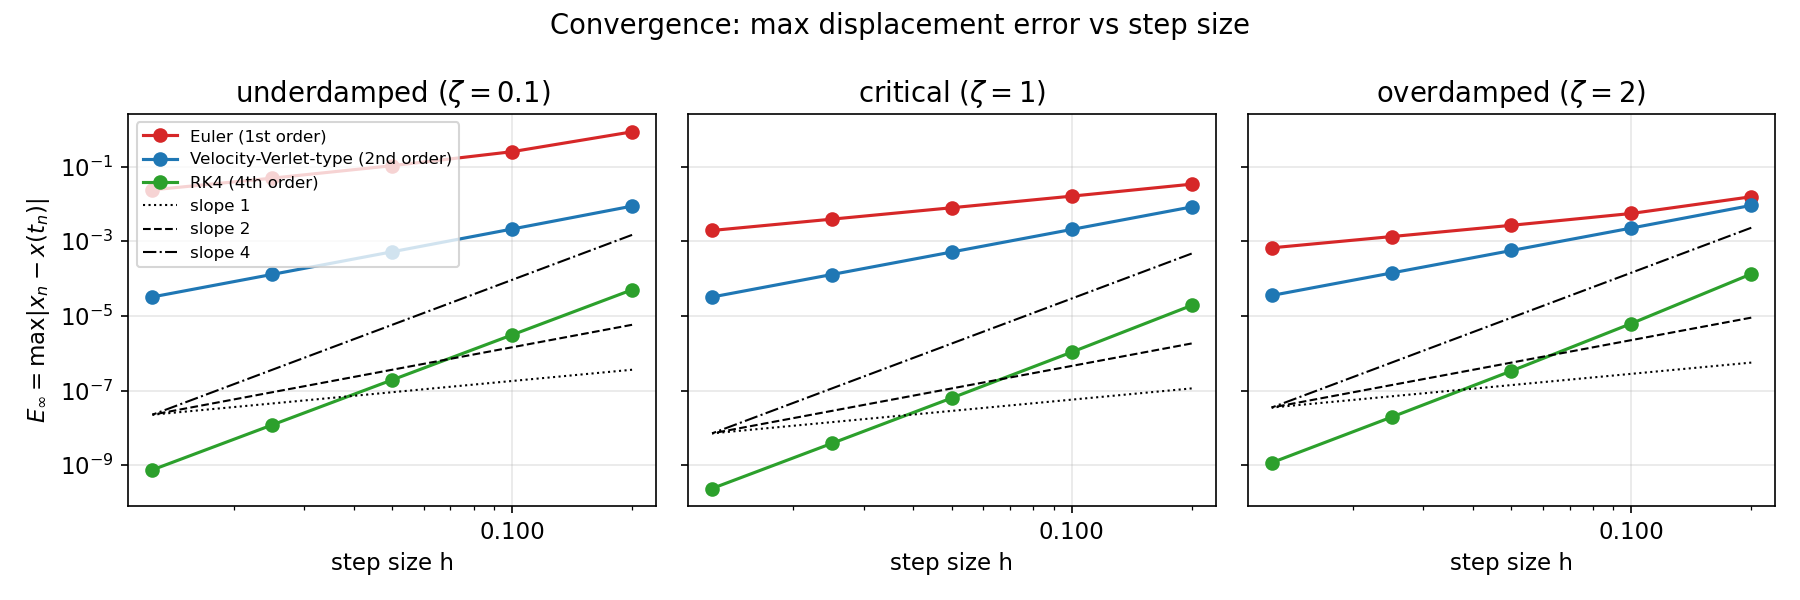
\includegraphics[width=\textwidth]{../paper_figures/fig4_convergence_loglog.png}
\caption{Maximum displacement error $E_\infty$ versus step size $h$
(log--log) for the three damping regimes, with reference slopes 1, 2,
and 4.}
\label{fig:conv}
\end{figure}

\begin{figure}[htbp]
\centering
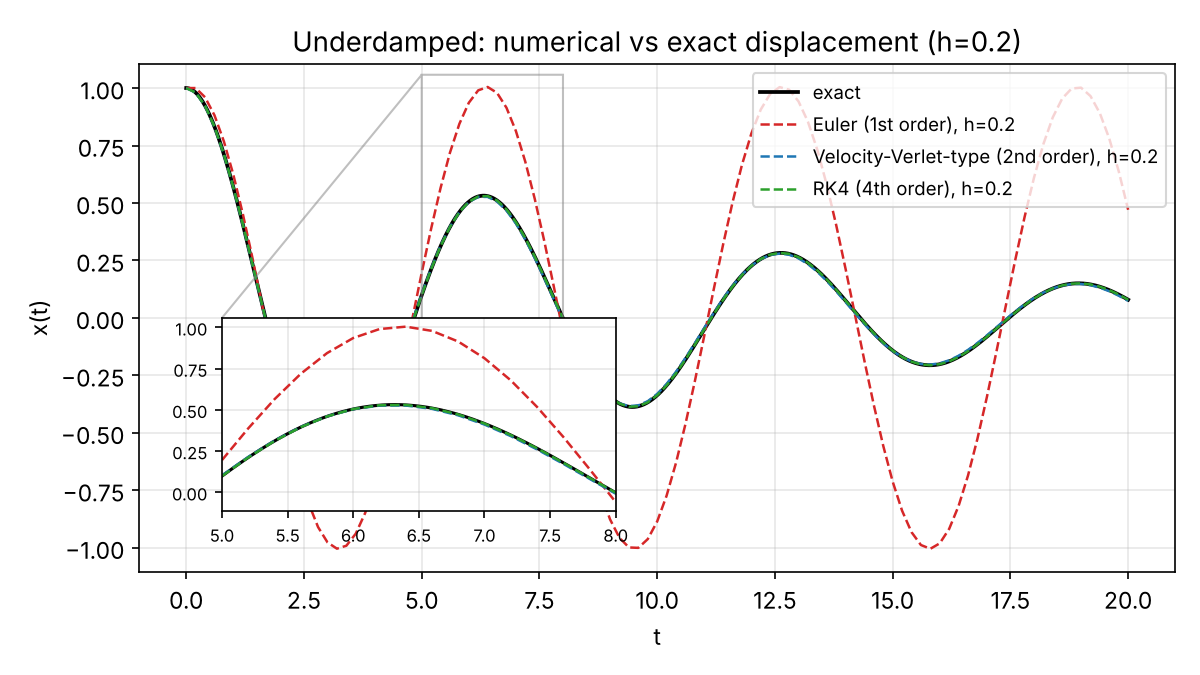
\includegraphics[width=\textwidth]{../paper_figures/fig1_underdamped_trajectory.png}
\caption{Underdamped ($\zeta=0.1$) displacement at $h=0.2$ with a zoomed
inset on the first peak. Euler does not decay; the Verlet-type and RK4
solutions overlay the exact curve.}
\label{fig:traj}
\end{figure}

On cost versus accuracy (Fig.~\ref{fig:cost}), RK4 dominates: at equal
wall-clock cost it is roughly $4$--$5$ orders of magnitude more accurate than
Euler where the measured costs overlap (e.g.\ at $\zeta=0.1$, for $\sim$0.9\,ms of compute, RK4 at
$h=0.05$ gives $E_\infty=1.9\times10^{-7}$ while Euler at $h=0.0125$
gives $2.4\times10^{-2}$). The Verlet-type scheme is the economical
middle ground; Euler is defensible only when very coarse accuracy
suffices. Timing is machine-dependent, so the exact positions in
Fig.~\ref{fig:cost} vary between runs.

\begin{figure}[htbp]
\centering
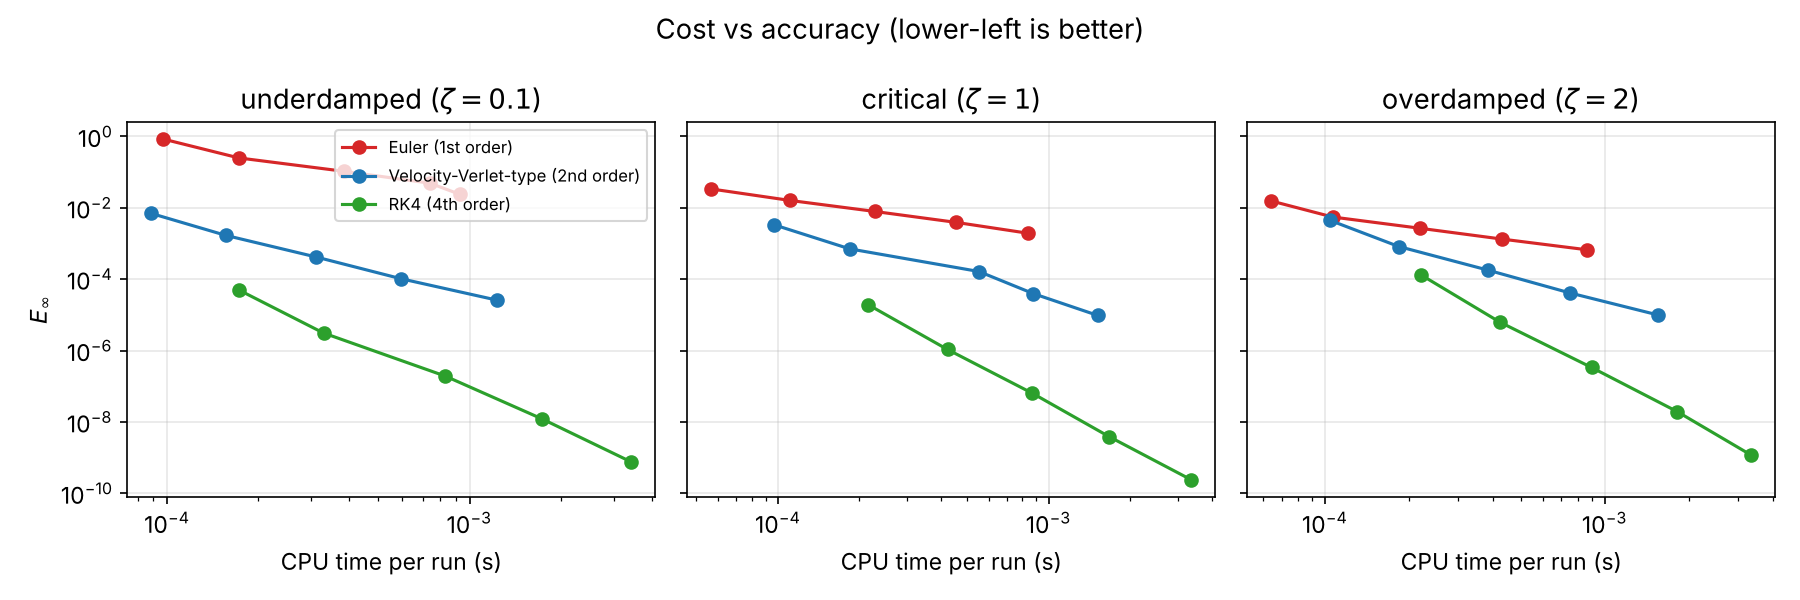
\includegraphics[width=0.85\textwidth]{../paper_figures/fig5_cost_vs_error.png}
\caption{Wall-clock cost versus $E_\infty$ at $\zeta=0.1$. RK4 gives
roughly $4$--$5$ orders of magnitude better accuracy at equal cost
where the measured costs overlap.}
\label{fig:cost}
\end{figure}

\subsection{Linear stability boundary}
\label{sec:stab}
For explicit Euler applied to the underdamped system, the eigenvalues
are $\lambda=-\zeta\pm i\omega_d$ and one step multiplies each
eigenmode by $1+h\lambda$, with squared modulus
\begin{equation}
|1+h\lambda|^2 = (1-h\zeta)^2 + h^2\omega_d^2
               = 1 - 2\zeta h + h^2.
\end{equation}
Stability ($|1+h\lambda|<1$) therefore requires $h<2\zeta$; at
$h=2\zeta$ the amplification factor is exactly 1 and the numerical
envelope neither grows nor decays. The discrete decay rate is
$\zeta_{\mathrm{disc}}=-\ln(1-2\zeta h+h^2)/(2h)$, so the predicted
relative envelope-decay error is
$|\zeta_{\mathrm{disc}}-\zeta|/\zeta$, which passes continuously through
$1$ ($100\%$) at $h=2\zeta$.

Figure~\ref{fig:stabscan} compares this prediction against the
independent fine scan at $\zeta=0.1$. The measured Euler errors run from
$0.799$ ($h=0.16$) through $1.000$ ($h=0.20$) to $1.248$ ($h=0.25$),
crossing $100\%$ exactly at the theoretical boundary; the largest
absolute deviation from the amplification-factor prediction over the
seven step sizes is $3.1\times10^{-5}$ (at $h=0.2$ the agreement is
$3.2\times10^{-6}$). The Verlet-type errors grow smoothly from
$0.0065$ to $0.0160$ and RK4 stays below $8\times10^{-5}$ (its small
nonmonotonic wiggles come from peak-fit noise, not from the integrator).

\begin{figure}[htbp]
\centering
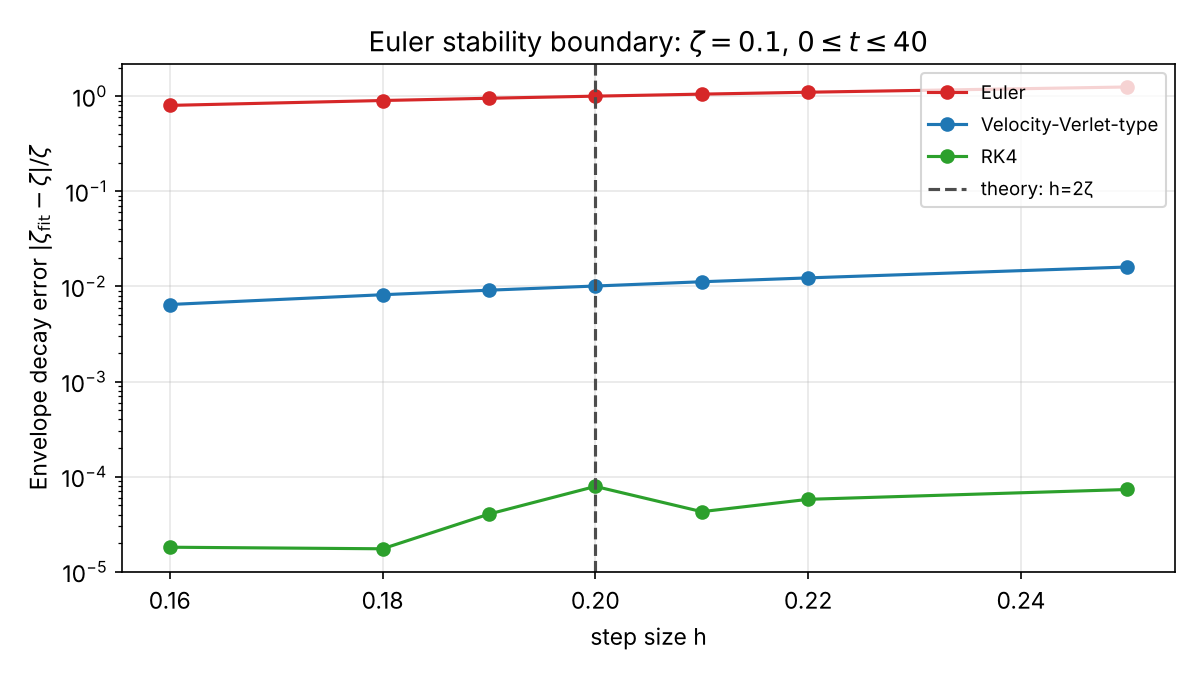
\includegraphics[width=0.85\textwidth]{../paper_figures/fig7_stability_boundary.png}
\caption{Fine scan of the Euler stability boundary at $\zeta=0.1$:
relative envelope-decay error versus $h$. The dashed line marks the
theoretical boundary $h=2\zeta=0.2$, where Euler's error passes through
$100\%$ (neutral numerical envelope).}
\label{fig:stabscan}
\end{figure}

Well beyond the boundary, at $h=0.5$, Euler blows up exponentially
($\max|x|=15$ on $t\in[0,20]$) while the other two schemes stay bounded
but visibly distorted (Fig.~\ref{fig:h05}).

\begin{figure}[htbp]
\centering
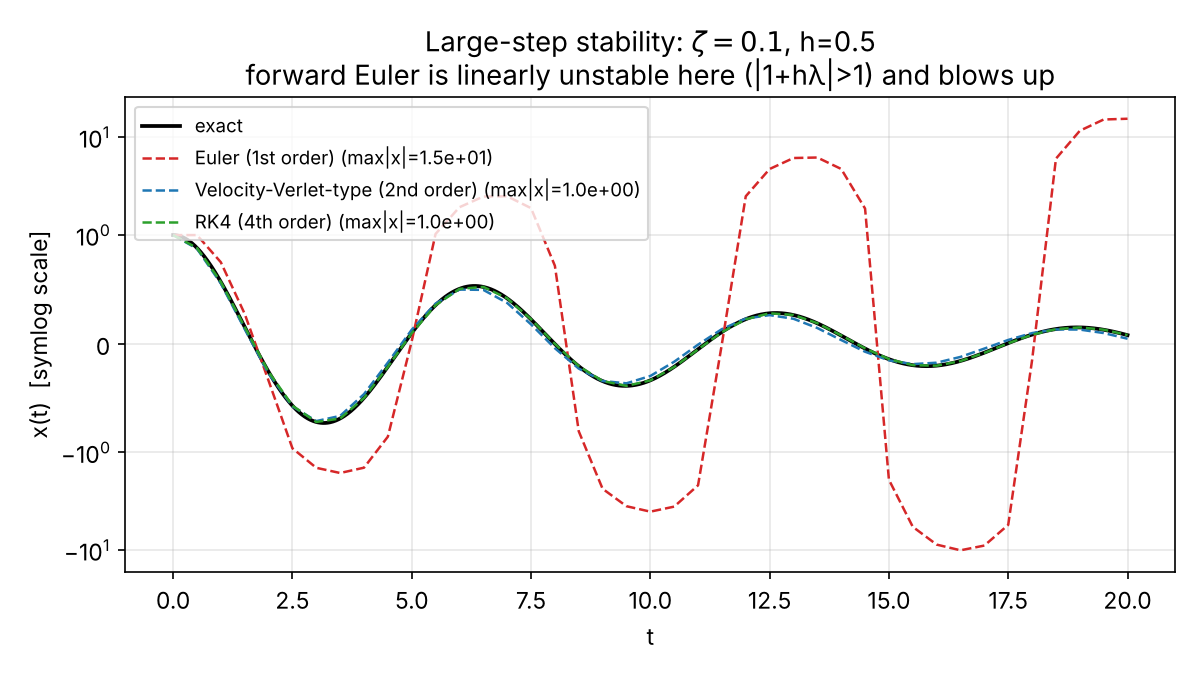
\includegraphics[width=0.85\textwidth]{../paper_figures/fig6_stability_h05.png}
\caption{Large-step behaviour at $\zeta=0.1$, $h=0.5$ (symlog scale):
Euler is linearly unstable and diverges; the Verlet-type and RK4
solutions stay bounded but are distorted.}
\label{fig:h05}
\end{figure}

\subsection{Long-time energy behaviour}
At $\zeta=0$ the exact energy $E_0=1/2$ is conserved, exposing each
scheme's secular behaviour over $t\in[0,100]$ (Fig.~\ref{fig:energy}).
Euler multiplies the energy by exactly $(1+h^2)$ per step:
\begin{equation}
\frac{E_n}{E_0} = (1+h^2)^n,
\end{equation}
so at $h=0.2$ ($n=500$ steps) the energy grows to
$(1.04)^{500}=3.286\times10^8$, matching the measured
$3.2860158\times10^8$ to all printed digits. Even at $h=0.1$ the growth
reaches $2.1\times10^4$.

At $\zeta=0$ the Verlet-type scheme reduces to standard velocity
Verlet (the acceleration no longer depends on $v$), and its relative
energy error is bounded and oscillatory with maximum $h^2/4$
(measured $0.0099998$ at $h=0.2$, i.e.\ $\sim$1\%; $0.0025$ at $h=0.1$).
RK4 has the smallest drift: its per-step energy multiplier is
$1-h^6/72+h^8/576$, giving a slow secular loss of only
$4.4\times10^{-4}$ at $h=0.2$ ($1.4\times10^{-5}$ at $h=0.1$).

\begin{figure}[htbp]
\centering
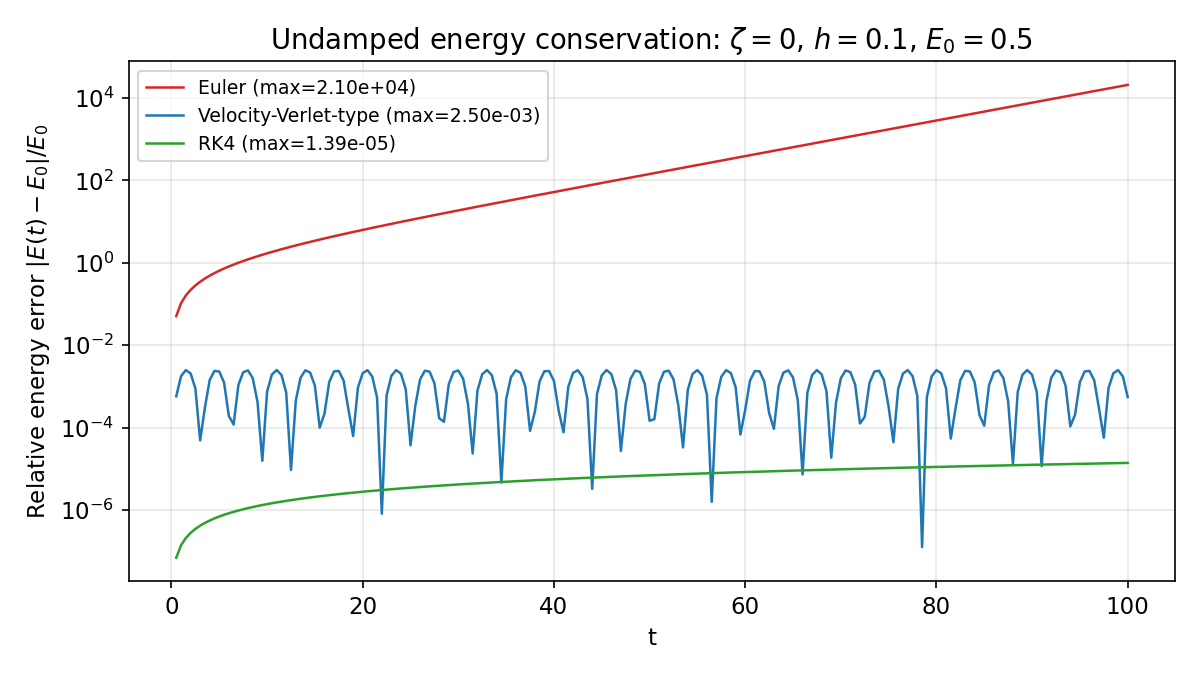
\includegraphics[width=0.85\textwidth]{../paper_figures/fig8_energy_drift.png}
\caption{Relative energy error $|E(t)-E_0|/E_0$ at $\zeta=0$, $h=0.1$,
$t\in[0,100]$ (log scale). Euler grows secularly; the Verlet-type error
is bounded and oscillatory; RK4 drifts the least. Legend maxima are
taken over the full integration grids.}
\label{fig:energy}
\end{figure}

\section{Discussion}
\paragraph{The Verlet-type scheme is not symplectic.}
We stress again (Section~\ref{sec:verlet}) that the scheme used here is
a pragmatic adaptation of velocity Verlet to velocity-dependent
damping, not the textbook symplectic algorithm. Its bounded energy
error in Fig.~\ref{fig:energy} comes from the fact that at $\zeta=0$ it
\emph{coincides} with standard velocity Verlet---not from any
symplectic property of the damped variant. For $\zeta>0$ no energy
conservation should be expected, and the second-order convergence in
Section~\ref{sec:conv} is the property that actually transfers.

\paragraph{Phase (dispersion) measurement limitation.}
The saved \texttt{metrics.csv} column \texttt{phase\_slope} holds
per-period peak-time drift. The implementation
(\texttt{analysis.phase\_error}) returns the least-squares slope;
the CSV values have been refreshed to match the corrected implementation.
A direct
recomputation from the saved trajectories at $\zeta=0.1$, $h=0.2$ with
parabolically refined peaks gives approximate drifts of
$-0.042$\,s/period (Euler), $-0.0097$\,s/period (Verlet-type), and
$+0.0003$\,s/period (RK4) against the exact period $T=6.315$\,s---but
with only three peaks in $t\in[0,20]$ these are coarse estimates, and we
present them as such.

\paragraph{Other limitations.}
The Euler convergence order at $\zeta=0.1$ ($1.27$) is steepened by the
pre-asymptotic $h=0.2$ point sitting on the stability boundary; it is
not evidence of superlinear convergence. RK4 at the finest step remains above machine epsilon; these runs do
not establish a round-off floor. CPU timings are machine-dependent. All figures are
regenerated from saved CSVs without re-running the solvers, so the
images are exactly reproducible from the repository data.

\section{Conclusion}
On the damped harmonic oscillator, textbook expectations are confirmed
quantitatively: explicit Euler is first-order, cheap per step, but
linearly unstable for $h>2\zeta$ and energetically disastrous over long
runs; the velocity-Verlet-type adaptation is robustly second-order and
an economical middle ground, though it must not be confused with
symplectic Verlet; classical RK4 is fourth-order and dominates on
accuracy per unit cost, with the smallest long-time energy drift. The
stability-boundary scan validates the linear theory
$|1+h\lambda|^2=1-2\zeta h+h^2$ to $3.1\times10^{-5}$, and the
energy-growth law $E_n/E_0=(1+h^2)^n$ for Euler is confirmed to machine
precision.

\paragraph{Data and reproducibility.}
All solvers (\texttt{solvers.py}), the analytic model
(\texttt{model.py}), the analysis (\texttt{analysis.py}), the experiment
runners (\texttt{experiments/}), the saved data (\texttt{data/*.csv}),
and the figure script (\texttt{figures/make\_figures.py}) are in the
local repository \texttt{damped-oscillator}. Figures were built
from the CSVs only; re-running the experiments reproduces the data
(modulo machine-dependent timings).

\end{document}
